\subsection{Cross-dataset transfer}
\label{sec:annotation}

\begin{table}[t]
\caption{mAP50--95 / counting MAE at confidence 0.25. Bold cells are in-domain.}
\label{tab:cross}
\centering
\begin{tabular}{lcc}
\toprule
Model & Laboro validation & tomatOD validation \\
\midrule
Laboro & \textbf{0.698 / 1.25} & 0.389 / 3.29 \\
tomatOD & 0.308 / 2.14 & \textbf{0.563 / 1.00} \\
Mixed & 0.704 / 1.14 & 0.546 / 1.24 \\
\bottomrule
\end{tabular}
\end{table}

Table~\ref{tab:cross} shows poor transfer in both directions for the
single-source models. The aggregate scores, however, combine two different
failure mechanisms. On tomatOD, the Laboro model retains a recall of 0.656,
compared with 0.879 for the tomatOD specialist. It therefore finds many of the
fruit but assigns them to the wrong stage. On Laboro, the tomatOD model falls to
a recall of 0.484 and undercounts every stage. The tomatOD result includes a
disagreement about maturity. The Laboro result is primarily a failure to find
fruit.

\begin{table}[t]
\caption{Per-stage counts on the tomatOD validation split at confidence 0.25.
Bias is the predicted total against the ground-truth total. An asterisk marks
the in-domain model.}
\label{tab:cross-stage}
\centering
\begin{tabular}{llrrr}
\toprule
Model & Stage & GT & predicted & bias \\
\midrule
Laboro   & green & 292 & 501 & $+72\%$ \\
         & half-ripened & 77 & 349 & $\mathbf{+353\%}$ \\
         & fully ripened & 99 & 49 & $\mathbf{-51\%}$ \\
\midrule
tomatOD$^{*}$ & green & 292 & 369 & $+26\%$ \\
         & half-ripened & 77 & 106 & $+38\%$ \\
         & fully ripened & 99 & 112 & $+13\%$ \\
\midrule
Mixed    & green & 292 & 398 & $+36\%$ \\
         & half-ripened & 77 & 114 & $+48\%$ \\
         & fully ripened & 99 & 135 & $+36\%$ \\
\bottomrule
\end{tabular}
\end{table}

Table~\ref{tab:cross-stage} separates the stage counts. On tomatOD, the Laboro
model predicts 4.5 times as many half-ripened fruit as are annotated and half as
many fully ripe fruit. Its green count is also inflated, as are the counts from
the other models at this threshold. The largest error is therefore a directed
substitution between the half-ripened and fully ripe stages. On its own split,
the tomatOD specialist over-predicts all three stages by between 13\% and 38\%.
This consistent inflation across stages indicates a threshold effect. The
in-domain Laboro result shows the same pattern (green $+10\%$, half-ripened
$+20\%$, fully ripened $+44\%$).

\begin{table}[t]
\caption{Fitted stage boundaries on median $a^*$, raw and after subtracting the
image background median. Self-recovery is the share of a dataset's own labels
its own two cuts reproduce. The swap rows apply one dataset's cuts to the
other's boxes and report the share of labels that change, overall and per
stage.}
\label{tab:colour-cuts}
\centering
\begin{tabular}{lrr}
\toprule
 & raw $a^*$ & background-corrected \\
\midrule
Laboro, cuts & $-10.1$, $+23.9$ & $+3.2$, $+31.0$ \\
\quad self-recovery & 82\% & 76\% \\
tomatOD, cuts & $-3.4$, $+6.3$ & $-0.1$, $+11.7$ \\
\quad self-recovery & 78\% & 78\% \\
\midrule
Laboro cuts on tomatOD & 64\% & 22\% \\
\quad green / half / fully & 71 / 1 / 97 & 1 / 25 / \textbf{98} \\
tomatOD cuts on Laboro & 16\% & 27\% \\
\quad green / half / fully & 1 / 77 / 9 & 20 / \textbf{75} / 7 \\
\bottomrule
\end{tabular}
\end{table}

\begin{figure*}[t]
  \centering
  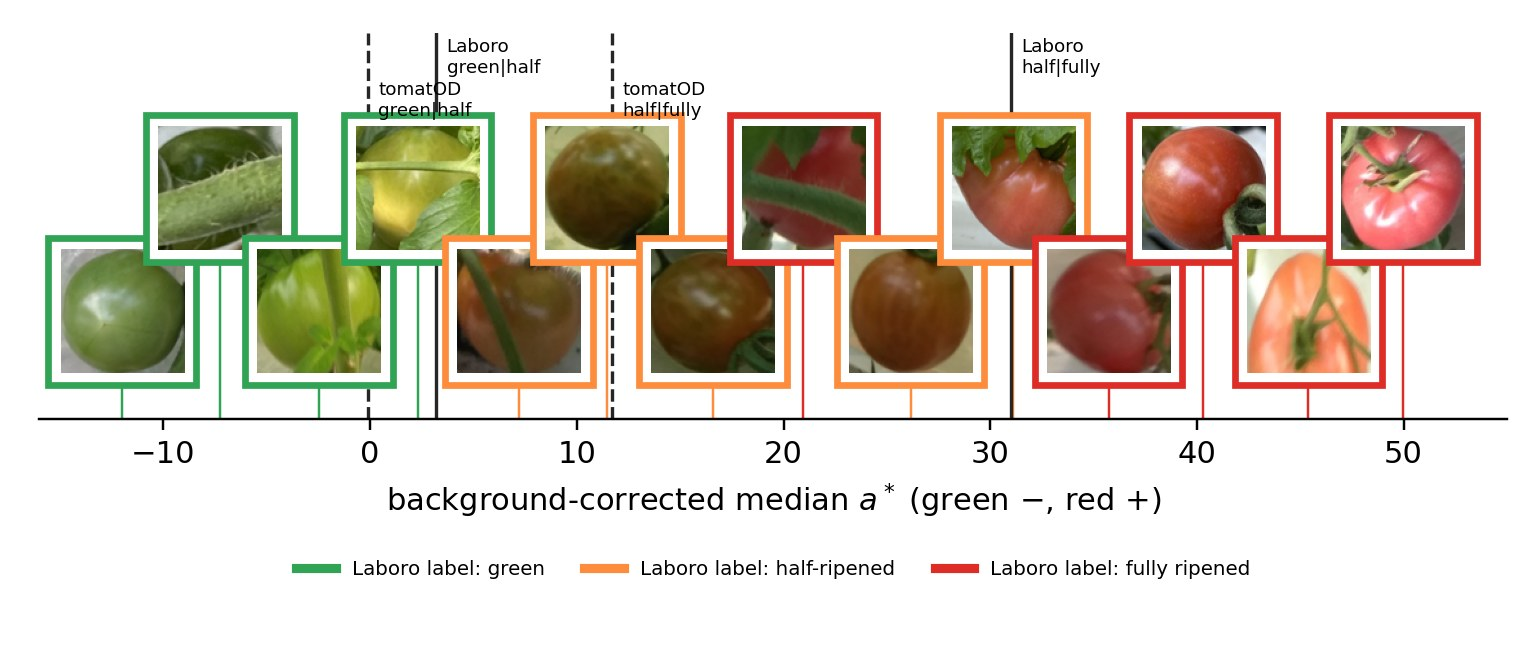
\includegraphics[width=0.85\textwidth]{colour_axis.jpg}
  \caption{Laboro validation fruit placed on the background-corrected $a^*$
  axis of Section~\ref{sec:colour}, framed in the colour of their Laboro label.
  Vertical lines are the stage boundaries fitted to each dataset
  (Table~\ref{tab:colour-cuts}): solid for Laboro, dashed for tomatOD. A fruit
  at $a^*\approx 20$ is half-ripened by Laboro's boundaries and fully ripe by
  tomatOD's. Examples were chosen to span the axis and to contain no
  neighbouring annotated fruit; tomatOD images are not shown.}
  \label{fig:colour-axis}
\end{figure*}

The colour measurement in Section~\ref{sec:colour} explains the direction of
this error. In Laboro, the median background-corrected $a^*$ values are $-5.6$
for green, $18.9$ for half-ripened, and $41.7$ for fully ripened fruit. In
tomatOD, the corresponding values are $-4.2$, $6.6$, and $13.6$. The datasets
therefore assign similar colours to the green stage. TomatOD assigns the fully
ripe label at a colour that Laboro assigns to the half-ripened stage. The gap
between the datasets grows from 12 points for the half-ripened stage to 28 for
the fully ripe stage. Figure~\ref{fig:colour-axis} illustrates these values with
real fruit.

The two fitted boundaries reproduce 76\% to 78\% of the labels in the dataset
from which they were derived (Table~\ref{tab:colour-cuts}). They therefore
provide a usable description of each annotation convention. Applying the
boundaries to the other dataset shows an asymmetric result. The Laboro
boundaries place 98\% of tomatOD's fully ripe boxes within Laboro's
half-ripened band, matching the substitution observed in the transfer counts.
In the other direction, the tomatOD boundaries move 75\% of Laboro's
half-ripened boxes into the fully ripe stage. The corresponding model-transfer
result does not show this disagreement because the tomatOD model first fails to
find many of the Laboro fruit.

The background correction separates the annotation difference from differences
in image capture. In the raw $a^*$ measurements, the two green medians differ by
10 points, $-17.7$ against $-7.8$. This difference is consistent with a change
in illumination or white balance. Subtracting the background median of each
image removes almost all of the green-stage gap. At the same time, it widens the
gap between the half-ripened and fully ripe stages. The remaining disagreement
after this per-image photometric normalisation is therefore associated with the
annotation conventions.

The detector trained on both datasets retains the two annotation conventions.
On Laboro, the mixed model matches the Laboro specialist (0.704 against 0.698
mAP50--95). On tomatOD, it is 0.017 below the tomatOD specialist. It also raises
the two cross-dataset results from 0.308 to 0.704 and from 0.389 to
0.546. The mixed model does not reproduce the Laboro model's stage bias on
tomatOD. The Laboro model gives a $-51\%$ fully ripe count, whereas the mixed
model gives $+36\%$. This is the same direction as the tomatOD specialist,
although Laboro supplies about 80\% of the training boxes. Because the two
source domains are visually distinguishable, the network can use a
source-conditional maturity boundary. Section~\ref{sec:discussion} considers
the implication of this result for label noise.

The counting column in Table~\ref{tab:cross} has a limitation that
Section~\ref{sec:calibration} measures. Those counts use a fixed confidence
threshold of 0.25.
Sweeping the threshold reduces the Laboro model's tomatOD counting error from
3.29 to 1.34. Thus, more than half of the apparent counting penalty under
transfer is associated with the selected operating point, which is the
confidence threshold used to produce the count. The mAP column is unaffected
because mAP integrates over confidence.

Converting both collections to one taxonomy also revealed two defects in the
published annotations. The tomatOD test split declares one category whose name
contains a list of all three stage names, while its annotation records use three
distinct category identifiers. Reading the categories separately for each
split therefore collapses the test split onto one class without an error. The
shipped annotations also contain 2,421 boxes, whereas the dataset documentation
reports 2,418. These defects do not affect the results above because the
experiments use the training and validation splits and map classes by name. A
name-based mapping exposes both defects, while an identifier-based mapping
would propagate them.
